\section{Experiments}
We compared the accuracy of four matching functionals, CC, MI, EM and ECC, all of them driving the SyN transformation model. We selected the CC functional because its robustness and accuracy for mono-modal registration have been demonstrated in large scale comparative studies \cite{Klein2009, Klein2010, Rohlfing2012} (it would be desirable to reach similar performance in the multi-modal case), we would like to quantify how large is its drop in accuracy for multi-modal images. MI \cite{Maes1997, Mattes2003} may be considered the functional of choice for multi-modal registration, it is expected that any new developed functional yields results at least as good as MI. The EM functional \cite{Arce-santana2014} is, to the best of our knowledge, the most recent proposal for multi-modal registration based on the assumption of a functional relationship between image modalities. It introduces a measure of uncertainty for each intensity, which may help to alleviate the effects of non-stationary relationships between image intensities. We implemented the EM functional to drive the SyN transformation model and extended it to make it symmetric (to estimate both transfer functions instead of only one), in our experiments, these modifications performed significantly better than the basic functional (non-symmetric, and using an elastic transformation model) proposed by Arce {\it et al.}\cite{Arce-santana2014}. Both MI and EM are voxel-wise functionals (i.e. it compares pairs of single voxels), while CC and ECC are computed from local rectangular windows.

\subsection{Mono-modal registration}
Although our matching functional was designed for multi-modal image registration, it is important to first verify that the quality of the algorithms is reasonable for mono-modal registration. Figure \ref{fig:mono_graph_seg} show the average overlap score for each of 31 manually annotated anatomical regions from the IBSR database. Note that the Jaccard indices obtained with CC (i.e. ANTS) are higher than reported by Rohlfing \cite{Rohlfing2012}. In his experiments, he used three resolutions with a maximum of 10, 10 and 5 iterations only. Here, we set a maximum of 100, 100 and 25 iterations, leaving the rest of the parameters unchanged (the same for all functionals). We can see that both MI and EM are very competitive, but still not as good as CC. This may be explained by the fact that CC uses a window centered at each voxel for computing the similarity, while MI and EM are voxelwise. By considering neighborhoods of the same size, the performance of ECC is practically the same as CC. 
%Table \ref{tab:monomodal_results_segTri_fill} shows the overlap scores over tissue types (white matter, gray matter and cerebrospinal fluid), instead of anatomical areas.
%Table \ref{tab:monomodal_results_seg} and
%% Table generated by Excel2LaTeX from sheet 'SyNEM-Monomodal-Large'
\begin{table}[htbp]
  {\small
  \centering
    \begin{tabular}{lcccc}
    \toprule
    \textbf{}& \textbf{SyN-EM} & \textbf{SyN-ECC} & \textbf{SyN-CC} & \textbf{SyN-MI} \\
    \midrule
    \textbf{Brain-Stem:} & 0.785898 & \textbf{0.81602} & 0.812225 & 0.804005 \\
    \textbf{Right-Cerebellum-Cortex:} & 0.736296 & \textbf{0.81515} & 0.813174 & 0.771044 \\
    \textbf{Left-Cerebellum-Cortex:} & 0.7393 & \textbf{0.81054} & 0.807955 & 0.765619 \\
    \textbf{Right-Thalamus-Proper:} & 0.714083 & 0.766215 & \textbf{0.77195} & 0.744856 \\
    \textbf{Left-Thalamus-Proper:} & 0.727093 & 0.762533 & \textbf{0.76732} & 0.74822 \\
    \textbf{Right-Putamen:} & 0.680673 & 0.747955 & \textbf{0.75095} & 0.711739 \\
    \textbf{Left-Putamen:} & 0.699259 & 0.744089 & \textbf{0.7444} & 0.721028 \\
    \textbf{Left-Cerebral-Cortex:} & 0.723987 & \textbf{0.7392} & 0.733487 & 0.687219 \\
    \textbf{Right-Cerebral-Cortex:} & 0.718819 & \textbf{0.7389} & 0.731013 & 0.683091 \\
    \textbf{Right-Cerebral-White-Matter:} & 0.702426 & \textbf{0.73313} & 0.720373 & 0.644731 \\
    \textbf{Left-Cerebral-White-Matter:} & 0.705485 & \textbf{0.73209} & 0.720678 & 0.646227 \\
    \textbf{Left-Lateral-Ventricle:} & 0.730771 & 0.727445 & \textbf{0.73152} & 0.717626 \\
    \textbf{Right-Lateral-Ventricle:} & 0.709368 & 0.71397 & \textbf{0.71718} & 0.699376 \\
    \textbf{Right-Cerebellum-White-Matter:} & 0.576438 & \textbf{0.70137} & 0.691481 & 0.607846 \\
    \textbf{Left-Cerebellum-White-Matter:} & 0.58125 & \textbf{0.70088} & 0.692959 & 0.611147 \\
    \textbf{Left-Caudate:} & 0.644992 & \textbf{0.67113} & 0.664751 & 0.666136 \\
    \textbf{Right-Caudate:} & 0.620211 & \textbf{0.6547} & 0.647248 & 0.651052 \\
    \textbf{Right-VentralDC:} & 0.612038 & 0.65134 & \textbf{0.65156} & 0.627547 \\
    \textbf{Left-VentralDC:} & 0.621505 & \textbf{0.65131} & 0.64987 & 0.631352 \\
    \textbf{Right-Pallidum:} & 0.497613 & \textbf{0.62173} & 0.620448 & 0.58236 \\
    \textbf{Right-Hippocampus:} & 0.572332 & \textbf{0.6209} & 0.62009 & 0.574656 \\
    \textbf{Left-Pallidum:} & 0.523736 & \textbf{0.61504} & 0.61357 & 0.583111 \\
    \textbf{Left-Hippocampus:} & 0.573814 & \textbf{0.61041} & 0.608895 & 0.563815 \\
    \textbf{4th-Ventricle:} & 0.55128 & 0.60626 & \textbf{0.6079} & 0.574298 \\
    \textbf{3rd-Ventricle:} & 0.526595 & 0.543999 & \textbf{0.54718} & 0.514933 \\
    \textbf{Left-Amygdala:} & 0.443793 & 0.518728 & \textbf{0.51924} & 0.483635 \\
    \textbf{Right-Amygdala:} & 0.41122 & 0.513423 & \textbf{0.51384} & 0.458386 \\
    \textbf{Left-Accumbens-area:} & 0.450545 & 0.499772 & \textbf{0.50044} & 0.461933 \\
    \textbf{Right-Accumbens-area:} & 0.432501 & 0.489832 & \textbf{0.49049} & 0.442778 \\
    \textbf{Right-Inf-Lat-Vent:} & 0.177488 & 0.229552 & \textbf{0.23206} & 0.161517 \\
    \textbf{Left-Inf-Lat-Vent:} & 0.189736 & 0.227756 & \textbf{0.233} & 0.166842 \\
    \bottomrule
    \end{tabular}}%
    \caption{Comparison of the registration performance (measured by the Jaccard index over 31 anatomical regions) of the Greedy SyN algorithm with EM, ECC, CC and MI metrics.
The Jaccard indices were averaged over 306 monomodal registrations. Top performer for each region is highlighted.}
  \label{tab:monomodal_results_seg}%
\end{table}%

%% Table generated by Excel2LaTeX from sheet 'SyNEM-Monomodal-Large'
\begin{table}[h!]
  \centering
  {\small
    \begin{tabular}{ccccc}
    \toprule
    \textbf{} & \textbf{ECC} & \textbf{CC} & \textbf{EM} & \multicolumn{1}{c}{\textbf{MI}} \\
    \midrule
    \textbf{Background}  & 0.995 & 0.995 & 0.994& \textbf{0.996} \\
    \textbf{CSF}         & 0.349 & 0.359 & 0.335& \textbf{0.370} \\
    \textbf{Gray Matter} & \textbf{0.765} & 0.759 & 0.740 & 0.717 \\
    \textbf{White Matter} & \textbf{0.739} & 0.728 & 0.703 & 0.654 \\
    \bottomrule
    \end{tabular}%
    \caption{{\small Comparison of the registration performance (measured by the Jaccard index over Background, CSF, GM and WM)of the Greedy SyN algorithm with ECC, CC, EM and MI metrics. The Jaccard indices were averaged over 306 monomodal registrations. Top performer for each region is highlighted.}}
  \label{tab:monomodal_results_segTri_fill}}%
\end{table}%


\begin{figure*}[t!]
\centering
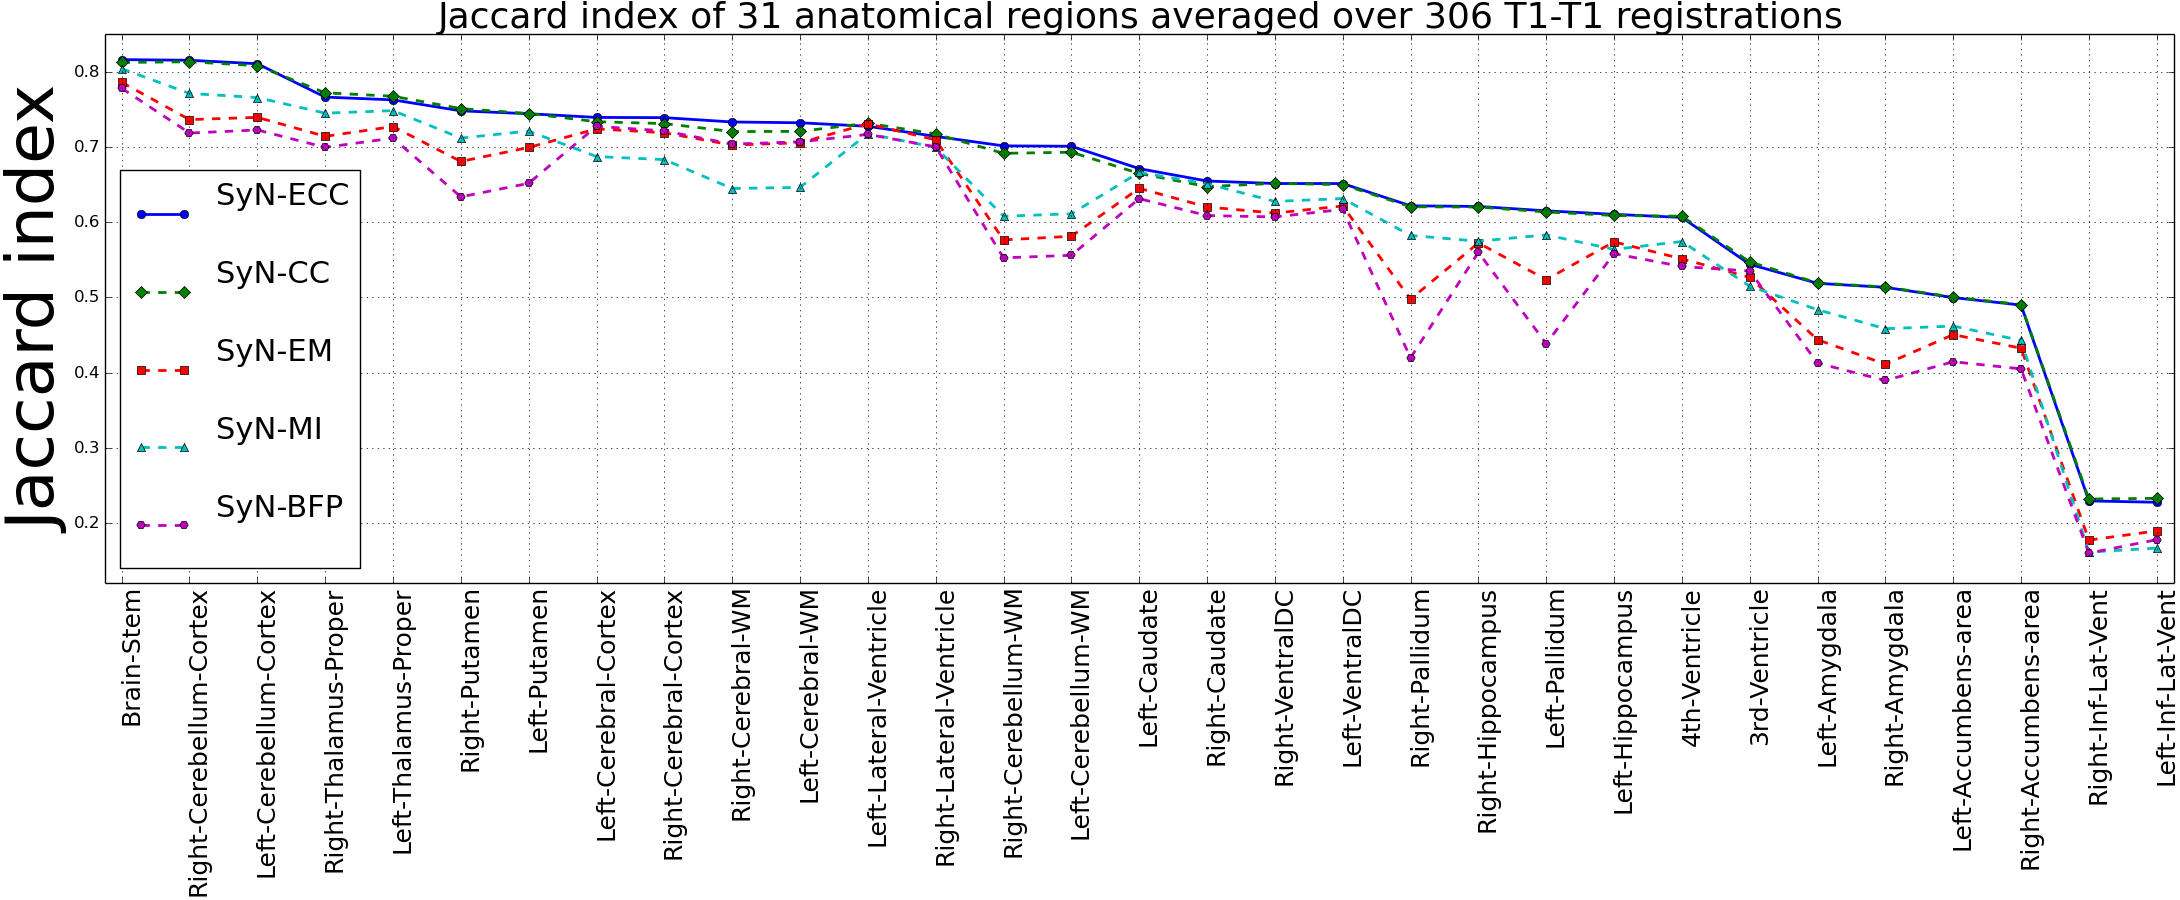
\includegraphics[width=1.0\linewidth]{./images/mono_lines_seg.png}\\
\caption{{\small Comparison of the registration performance (measured by the Jaccard index over 31 anatomical regions) of the Greedy SyN algorithm with EM, ECC, CC and MI metrics. The Jaccard indices were averaged over 306 monomodal registrations.}}
\label{fig:mono_graph_seg}\figcloser
\end{figure*}

\subsection{Multi-modal registration}\label{sec:multimodal_results}

To assess accuracy in the multi-modal case, we generated synthetic T2 images for all IBSR T1 images as follows. We first register the Brainweb T1 template (which plays the role of moving image) towards each IBSR T1 image (which play the role of fixed images) using ANTs with the CC metric (a mono-modal registration problem, where we know that ANTS with CC performs remarkably well). Then we applied the resulting deformation field to the Brainweb T2 template. The transfer function from the real T1 image to the warped T2 template is computed as the average T2 intensity associated to each T1 intensity. The computed transfer function is then applied to the real IBSR T1 image obtaining a ``perfectly aligned'' realistic synthetic T2 image for each IBSR volume, therefore the annotations remain exactly the same as the T1 counterparts and we are able to compute the overlap scores as before. Note that the number of registrations we need to perform is now 612 because we can use the T2 modality either as the moving or the fixed image. It is very important to note that, although the way we generate the semi-synthetic images may appear to be tailored towards our model (the so-called ``inverse crime''), this is not the case. Please note that intensities of each real image are transformed using a different transfer function, which maps intensities to each warped template. The warped templates are simply discarded afterwards, and not used for evaluation any more. Images from the same subject (real and synthetic) are never registered to each other during evaluation. Therefore, there will not exist, in general, any transfer function mapping intensities between any pair of images registered during validation. Figure \ref{fig:multi_seg} shows results similar to Figure \ref{fig:mono_graph_seg} but this time averaged over 612 multimodal registrations. Note how the performance of the CC metric strongly drops while EM, ECC and MI are less affected by the change of modality.\\

The Brainweb template also provides us with a simulation of a proton density (PD) image for the same brain anatomy. This allows us to repeat the procedure described above for each pair of three modalities, T1, T2 and PD. Figure \ref{fig:all_pairs_boxplots} depicts a summary of the results obtained over all pairs of modalities. For each pair of registered images, we compute the average Jaccard index of all anatomical regions. Each boxplot in Figure \ref{fig:all_pairs_boxplots} corresponds to the set of all 306 (mono-modal) or 612 (multi-modal) average scores for that particular method and that particular pair of modalities. We can observe that the CC metric performs very well for all mono-modal experiments (diagonal graphs), but it is severely affected in the multi-modal case (off-diagonal graphs). The ECC metric performs practically the same as CC in the mono-modal case, but is less affected in the multi-modal case.
%Table \ref{tab:multimodal_results_segTri_fill} shows the overlap scores of tissue types, where the same behavior can be observed.\\
%Table \ref{tab:monomodal_results_seg} and
%Table \ref{tab:multimodal_results_seg} and
%\begin{figure}[H]
%\centering
%    \includegraphics[width=\linewidth]{./images/semi_synthetic_image_creation.png}
%    \caption{{\small Semi-synthetic, manually annotated images for quantitative evaluation of multi-modal non-linear image registration algorithms.}}
%\label{fig:semi_synthetic_image_creation}
%\end{figure}
%% Table generated by Excel2LaTeX from sheet 'SyNEM-Multi-Large'
\begin{table}[htbp]
\begin{adjustwidth}{-0.75cm}{}
  \centering
  {\small
    \begin{tabular}{lcccc}
    \toprule
          & \textbf{SyN-EM} & \textbf{SyN-ECC} & \textbf{SyN-CC} & \textbf{SyN-MI} \\
    \midrule
    \textbf{Brain-Stem} & 0.786 & \textbf{0.812} & 0.663 & 0.792 \\
    \textbf{Right-Cerebellum-Cortex} & 0.729 & \textbf{0.801} & 0.645 & 0.757 \\
    \textbf{Left-Cerebellum-Cortex} & 0.729 & \textbf{0.796} & 0.649 & 0.751 \\
    \textbf{Right-Thalamus-Proper} & 0.716 & 0.755 & \textbf{0.756} & 0.738 \\
    \textbf{Left-Thalamus-Proper} & 0.727 & \textbf{0.754} & 0.752 & 0.737 \\
    \textbf{Right-Putamen} & 0.684 & \textbf{0.738} & 0.676 & 0.703 \\
    \textbf{Left-Putamen} & 0.699 & \textbf{0.735} & 0.683 & 0.711 \\
    \textbf{Left-Cerebral-Cortex} & 0.699 & \textbf{0.716} & 0.558 & 0.658 \\
    \textbf{Right-Cerebral-Cortex} & 0.694 & \textbf{0.714} & 0.548 & 0.653 \\
    \textbf{Left-Lateral-Ventricle} & 0.706 & 0.713 & \textbf{0.733} & 0.665 \\
    \textbf{Right-Cerebral-White-Matter} & 0.683 & \textbf{0.710} & 0.571 & 0.610 \\
    \textbf{Left-Cerebral-White-Matter} & 0.685 & \textbf{0.710} & 0.570 & 0.612 \\
    \textbf{Right-Lateral-Ventricle} & 0.687 & 0.696 & \textbf{0.718} & 0.643 \\
    \textbf{Right-Cerebellum-White-Matter} & 0.579 & \textbf{0.688} & 0.476 & 0.600 \\
    \textbf{Left-Cerebellum-White-Matter} & 0.582 & \textbf{0.685} & 0.485 & 0.601 \\
    \textbf{Left-Caudate} & 0.628 & \textbf{0.646} & 0.637 & 0.645 \\
    \textbf{Left-VentralDC} & 0.622 & \textbf{0.644} & 0.491 & 0.620 \\
    \textbf{Right-VentralDC} & 0.616 & \textbf{0.644} & 0.499 & 0.617 \\
    \textbf{Right-Caudate} & 0.606 & 0.628 & 0.618 & \textbf{0.635} \\
    \textbf{Right-Hippocampus} & 0.570 & \textbf{0.607} & 0.503 & 0.557 \\
    \textbf{Right-Pallidum} & 0.528 & \textbf{0.602} & 0.499 & 0.579 \\
    \textbf{4th-Ventricle} & 0.546 & \textbf{0.599} & 0.543 & 0.549 \\
    \textbf{Left-Pallidum} & 0.545 & \textbf{0.598} & 0.495 & 0.576 \\
    \textbf{Left-Hippocampus} & 0.567 & \textbf{0.596} & 0.488 & 0.544 \\
    \textbf{3rd-Ventricle} & 0.511 & \textbf{0.535} & 0.492 & 0.482 \\
    \textbf{Left-Amygdala} & 0.447 & \textbf{0.509} & 0.360 & 0.479 \\
    \textbf{Right-Amygdala} & 0.415 & \textbf{0.498} & 0.339 & 0.457 \\
    \textbf{Left-Accumbens-area} & 0.448 & \textbf{0.487} & 0.338 & 0.449 \\
    \textbf{Right-Accumbens-area} & 0.433 & \textbf{0.476} & 0.339 & 0.425 \\
    \textbf{Right-Inf-Lat-Vent} & 0.164 & \textbf{0.215} & 0.178 & 0.146 \\
    \textbf{Left-Inf-Lat-Vent} & 0.178 & \textbf{0.214} & 0.194 & 0.151 \\
    \hline
    \textbf{Average (std.)} & 0.587 (0.146) & 0.630 (0.142) & 0.532 (0.148) & 0.585 (0.147) \\
    \textbf{Rank-1 count} & 0 & 27 & 3 & 1 \\
    \textbf{Rank-2 count} & 9 & 4 & 3 & 15 \\
    \textbf{Rank-3 count} & 18 & 0 & 3 & 10 \\
    \bottomrule
    \end{tabular}}%
    \caption{Comparison of the registration performance (measured by the Jaccard index over 31 anatomical regions) of the Greedy SyN algorithm with EM, ECC, CC and MI metrics.
The Jaccard indices were averaged over 612 multimodal registrations. Rank-$k$ counts show the number of anatomical regions for which each
method ranked $k$ among the four methods under comparison. Top performer (rank-1) for each region is highlighted.}
  \label{tab:multimodal_results_seg}%
\end{adjustwidth}
\end{table}%

%% Table generated by Excel2LaTeX from sheet 'Sheet1'
\begin{table}[htbp]
  \centering
  \caption{Add caption}
    \begin{tabular}{|r|r|r|}
    \toprule
    \textbf{} & \textbf{SyN-ECC} & \textbf{SyN-CC} \\
    \midrule
    \textbf{Background} & 0.99074 & 0.99047 \\
    \textbf{CSF} & 0.21598 & 0.15738 \\
    \textbf{Gray Matter} & 0.72508 & 0.59738 \\
    \textbf{White Matter} & 0.72817 & 0.57185 \\
    \bottomrule
    \end{tabular}%
  \label{tab:addlabel}%
\end{table}%


\begin{figure*}[t!]
\centering
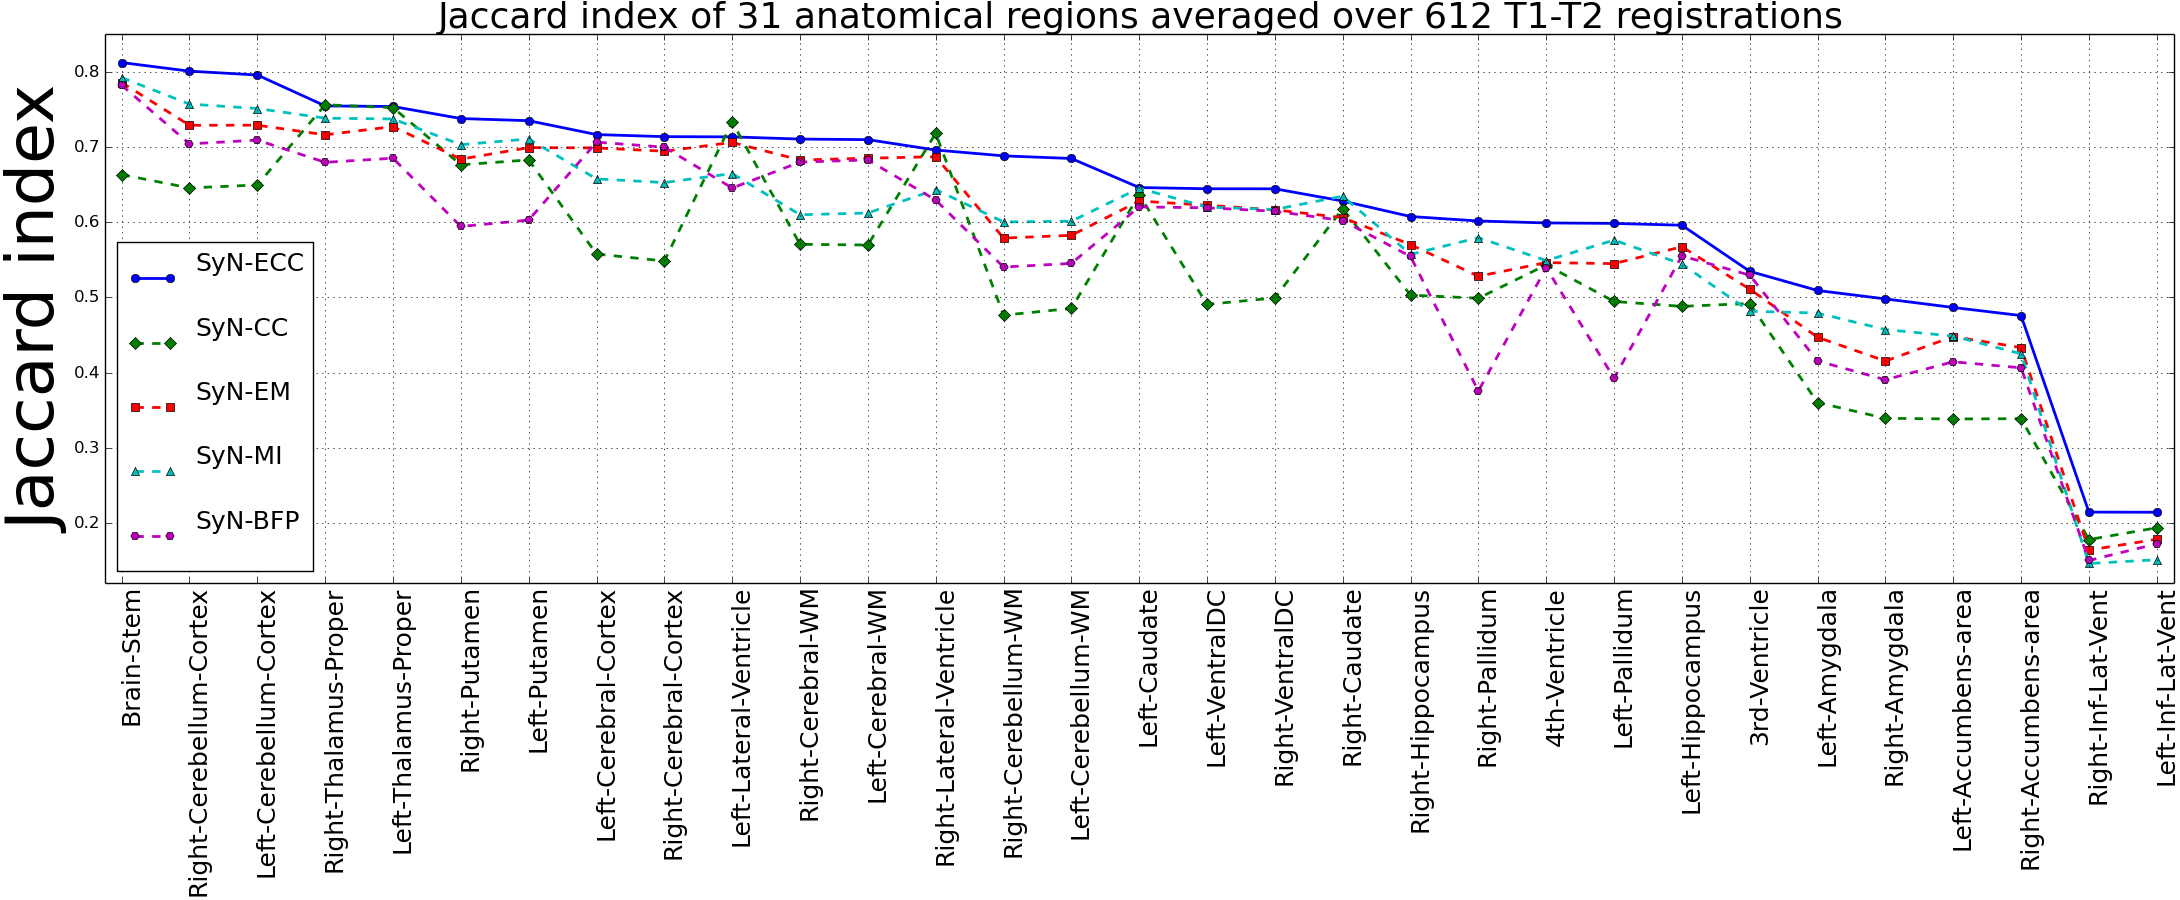
\includegraphics[width=1.0\linewidth]{./images/multi_lines_seg.png}\\
\caption{{\small Comparison of the registration performance (measured by the Jaccard index over 31 anatomical regions) of the Greedy SyN algorithm with EM, ECC, CC and MI metrics. The Jaccard indices were averaged over 612 multimodal registrations.}}
\label{fig:multi_seg}\figcloser
\end{figure*}

\begin{figure}[t!]
\centering
    \includegraphics[width=\linewidth]{./images/all_modality_pairs_boxplots.png}
    \caption{{\small Distributions of average Jaccard indices for all pairs of available modalities (T1, T2 and PD). For each pair of registrations, we compute the average Jaccard index of all anatomical regions.}}
\label{fig:all_pairs_boxplots}\figcloser
\end{figure}

\subsection{$B_{0}$-T1 registration}
Quantitative results shown in previous section indicate that ECC and MI perform best for multi-modal registration. Fig. \ref{fig:comparison_B0_T1_coregistration} depicts a a $B_{0}$-T1 registration result obtained using ECC and MI. We can see from the level curves that the result obtained with ECC matches better the local structure of the T1. This behavior is explained by the fact that the ECC functional is computed over local windows rather than single voxel pairs. Since a realistic T1-$B_{0}$ template is not available, the validation methodology described in previous section cannot be used to validate $B_{0}$-T1 registration. Instead, we performed an indirect quantitative validation as follows. We first register the $B_{0}$ (moving) image towards each T1 (fixed) annotated image, obtaining diffeomorphisms $\phi_{i}$, $i=1,2,...,18$. Then, for every pair $\phi_{i}, \phi_{j}$, we compute the composition $\phi_{i,j}:=\phi_{i}\circ \phi_{j}^{-1}$ (which now maps two annotated T1 images). The resulting overlap score indirectly measures the (combined) accuracy of both transforms. Quantitative results of the indirect validation are depicted in fig. \ref{fig:indirect_validation_boxplots}. We can see that the average Jaccard index obtained with ECC is higher (and with lower variance) than using any of the other matching functionals, which also demonstrates the ECC robustness.
%\begin{figure}[p]
%\centering
%    \subfloat[Example $B_{0}$-T1 registration result using SyN with %ECC.]{\label{fig:epicor_b0up_ecc}\includegraphics[width=1.0\linewidth]{./images/T1B0Result/epicor_b0up_ecc.png}}\\
%    \subfloat[Example $B_{0}$-T1 registration result using SyN with MI.]{\label{fig:epicor_b0up_mi}\includegraphics[width=1.0\linewidth]{./images/T1B0Result/epicor_b0up_mi.png}}
%    \caption{{\small Example of a $B_{0}$-T1 registration result using SyN with ECC and MI. Level curves of the warped $B_{0}$ were overlaid on top of the (undeformed) T1 to %visually assess local structure agreement. Visually, level curves obtained with ECC have a better correspondence with the structure of the T1. This visual assessment is confirmed %quantitatively, as shown in fig. \ref{fig:indirect_validation_boxplots}.}}
%\label{fig:comparison_B0_T1_coregistration}
%\end{figure}


\begin{figure}[t!]
\centering
    \subfloat[]{\label{fig:epicor_b0up_ecc}\includegraphics[width=0.5\linewidth]{./images/T1B0Result/epicor_b0up_ecc_mi_slim.png}}
    \subfloat[]{\label{fig:indirect_validation_boxplots}\includegraphics[width=0.30\linewidth]{./images/T1B0Result/jaccard_boxplots_T1_B0_slim.png}}
    \caption{{\small $B_{0}$-T1 registration results. (a) Example result using SyN with ECC (top) and MI (bottom). Level curves of the warped $B_{0}$ were overlaid on top of the T1 to visually assess local structure agreement. Visually, level curves obtained with ECC have a better correspondence with the structure of the T1. (b) Visual assessment from panel (a) is confirmed by the quantitative results using the indirect validation procedure (see text).}}
\label{fig:comparison_B0_T1_coregistration}\figcloser
\end{figure}
%\begin{figure}[H]
%\centering
%    \includegraphics[width=\linewidth]{./images/T1B0Result/jaccard_boxplots_T1_B0.png}
%    \caption{{\small $B0$-T1 registration results using the indirect validation procedure (see text).}}
%\label{fig:indirect_validation_boxplots}
%\end{figure}

%\begin{figure}[H]
%\centering
%    \includegraphics[width=\linewidth]{./images/new_validation.png}
%    \caption{{\small Indirect validation protocol for $B_{0}$-T1 registration.}}
%\label{fig:indirect_validation}\figcloser
%\end{figure}


